\section{Microarchitectural Timing Channels, Sources and Solutions}
Figure \ref{fig:baseline} shows a baseline architecture that is vulnerable to 
timing channels. It has multiple cores each with a branch predictor, core 
logic, a TLB, and one or more private caches. A trusted software layer (such as 
an operating system) allocates software entities (such as processes) to the 
cores. Software entities may be time multiplexed on cores (e.g. by context 
switching), but only one software entity may reside on a core at a time. The 
cores are connected to a shared cache via an on chip network. A shared system 
bus connects the shared cache to a memory controller that manages requests to 
main memory.
    \begin{figure}
        \begin{center}
            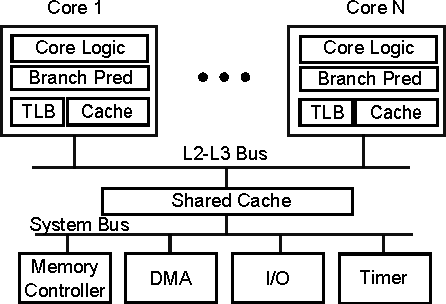
\includegraphics[width=1.62in]{figs/baseline.pdf}
            \caption{The timing-channel vulnerable baseline architecture.}
            \label{fig:baseline}
        \end{center}
    \end{figure}

The multicore system of interest consists of hardware resources that are
concurrently shared by multiple software entities. It is possible for software 
entities to be time multiplexed on the same core (e.g.  by context switching 
VMs), but the system does not allow software entities to execute concurrently 
on the same core (e.g. through simultaneous multithreading). 

Many microarchitectural timing channels and corresponding solutions are 
well-known. Shared caches create a state-based timing channel where interfering 
entities cause cache block replacements. This can be prevented by partitioning 
the cache among the entities. On chip networks and buses have contention based 
timing channel since only one entity can use the bus at a time. Time division 
multiplexing can resolve this issue \cite{yaonocs}. The authors of 
\cite{ushpca14} have exposed contention based and state based timing channels 
in the main memory and memory controller. They propose time division 
multiplexing the memory controller, partitioning the memory controller queueing 
structure, and using a closed-page row buffer management policy to close these 
timing channels. Finally, the private, per-core resources of the system such as 
the branch predictors, TLBs and private caches also create timing channels 
since software entities share cores through time multiplexing (for example, 
processes may be context switched in and out of the same core). These can be 
resolved by flushing the state elements of these resources on before moving a 
new software entity onto the core.

One could envision a straightforward approach to eliminating timing channels 
that simply combines all of these known approaches. However, this is not 
enough. Without carefully coordinating time multiplexed components, the system 
is subject to unnecessarily high overheads or total starvation.  Further, we 
expose three new microarchitectural timing channels that are not addressed by 
known solutions. The rest of this section develops a unified framework for 
identifying solutions to microarchitectural timing channels based on the 
taxonomy. It then details the timing channel vulnerabilities of the baseline 
architecture and corresponding solutions.

\subsection{General Approaches}

% Moved from the taxonomy. Need to be cleaned up.

Internal microarchitectural timing channels can either be state based, or 
contention based. In a \emph{state based} timing channel, the victim and 
adversary share some hardware state element with access timing that depends on 
its contents. Conventional shared caches have state based timing channels; 
accesses to memory addresses in the cache are faster than those that are not.
In a \emph{contention based} timing channel, the victim and adversary share a 
resource that can handle only a finite number of requests at a time.  Requests 
made to the resource while it is already handling a request are delayed. 
Conventional buses have contention based timing channels since a finite number 
of requests can be transferred at a time while the remaining requests are 
delayed in a queue.

%% Not sure if the covert channel paragraph is needed
We show how this taxonomy can be used to identify general approaches to prevent 
each type of timing channel in Section \ref{sec:tc_sources}. Though the use of 
a victim and an adversary in these definitions may seem to limit this taxonomy 
to timing side channels, it is equally valid for categorizing timing covert 
channels. To categorize covert channels, the victim is replaced with an 
adversary that intentionally sends messages to a second adversary through the 
timing channel.

The classification of a timing channel in the taxonomy can be used to identify 
a general solution to resolving the timing channel. This is useful for applying 
timing channel protection to new components not present in our baseline.  
\subsubsection{State Based Timing Channels}
Caches, TLBs, and branch predictors all have state based timing channels. In 
each, requests that use an entry that is present in the state elements (e.g.  
cache hits) are faster than requests to entries not present (e.g. cache 
misses). The state elements can contain a finite number of entries, so entries 
must be evicted and replaced with new ones. One software entity can evict 
entries owned by another, causing interference and timing channel leakage if 
the choice of entries evicted correlates with a secret. Generally, state based 
timing channels can be closed by applying flattening, partitioning, or 
flushing.

Flattening eliminates the dependence of access time on the state by forcing 
every access to take the same amount of time. For some components, this is a 
brute-force approach. Applied to caches, every access must be treated as a 
misss, so this is equivalent to removing the cache. However, for some 
vulnerable components, such as the row buffers of main memories, this is the 
most sensible approach.

Partitioning prevents software entities that share state elements from 
interfering. Static partitioning is realized by dividing the state elements 
into separate partitions for each software entity. Entities are only allowed to 
evict entries within their own partitions. Partitions must either be static, or 
at least not resized or moved based on the dynamic behaviour of an entity.
% If a partition is increased for an entity intensively using the state 
% elements, the other entities can detect that their partitions have been 
% resized and information is leaked.
However, partitions do not need to be heterogeneous and can be sized according 
to static performance characterizations of each software entity (assuming this 
information can be made public).

Flushing can be applied to state based resources that are shared only through 
time multiplexing (such as private caches shared through context switches).  At 
the end of a time quantum, the state elements are completely cleared before 
passing ownership of the state elements to the entity in the next time quantum.  
Resources that can be flushed can also be partitioned, and there are tradeoffs 
between these approaches.
% Flushing increases the time wasted at the end of a time quantum if flushing 
% cannot be done in less than one clock cycle. Clearing the state between time 
% quanta also increases the number of slower accesses at the start of the 
% quanta (e.g. it causes more cold cache misses). However, partitioning reduces 
% the total number of state elements that can be allocated to each entity. 
If the time quanta are longer (e.g. if context switching is infrequent), 
flushing is preferable to increase the total usable space, but partitioning may 
offer better performance for shorter time quanta by eliminating the time needed 
to flush and lessening the cold misses.

\subsubsection{Contention Based Timing Channels}
Contention based timing channels arise whenever a resource that is shared among 
multiple software entities can only handle a finite number of requests at a 
time. Contention based timing channels can be resolved by either duplication or 
time division multiplexing (TDM). In some cases, it may be possible to resolve 
contention for a resource by simply adding duplicate resources for each 
software entity. However, this has obvious area overhead implications. If 
duplication is infeasible, time division multiplexing should be used. TDM 
defines a schedule where each software entitiy is guaranteed a period of time, 
called a time quantum, where only that entity can use the resource. The 
schedule of time quanta must either be static or at least independent of the 
dynamic behavior of software entities.

\subsubsection{External Timing Channels}
Though timing channels external to hardware are outside the scope of this 
paper, there are a class of timing channels that are internal to hardware, but 
appear as external timing channels between two software entities. This form of 
external timing channel exists in systems where distrusting software entities 
must communicate. For example, one software entity might be a user space 
process and another might be a process that performs only high-assurance 
operations. The user space process requests the high-assurance process to 
perform some operation on its behalf. The user space process can directly 
observe the execution time of the other process. This type of timing channel 
can be solved in software by forcing the observable execution time to wait 
until the worst case time is reached.

\subsection{Microarchitectural Timing Channels and Solutions}
We now describe the specific timing channel vulnerabilities of the baseline 
architecture and show how these generalized approaches can be adapted to solve 
each individual timing channel.
\subsubsection{Shared Caches}
The shared caches of the baseline have a state based timing channel. Requests 
to the memory hierarchy for addresses that are stored in the cache (cache hits) 
are returned faster than requests for entries not stored in the cache (cache 
misses). So, the time required to access the cache depends on its state. The 
cache can only accommodate a finite number of entries, so when new entries must 
be stored, old ones are evicted. One software entity can evict the entries of 
another, causing timing channel leakage.

This state based timing channel should be closed by partitioning the cache 
among the timing compartments. At least two cache partitioning techniques 
exist: way partitioning and set partitioning 
\cite{rtas_cache_framework,dynamic_partitioning}. Set associative caches divide 
the cache into ways. Each way as a single slot for each cache set. A cache 
block may be stored in any way, but the set it belongs to is determined by a 
segment of its address bits called the index. Since many addresses are mapped 
to the same set, another segment of the address, the tag, is used to detect 
cache hits (i.e. if a specific address is present in the cache).

Way partitioning allocates a subset of the ways to each entity 
\cite{citation_needed}. This results in a reduction in the effective 
associativity utilized by each entity, and thus, causes more conflict misses 
and weakens performance. Set partitioning manipulates virtual to physical 
address translation to restrict the sets that a particular entity can occupy.  
When done at the granularity of a page, this is called page coloring, and this 
has been proposed for performance \cite{citation_needed} and real-time systems 
\cite{rtas_cache_framework}.  Although both techniques increase the number of 
capacity misses, set partitioning does not increase the number of conflict 
misses, so we chose this technique for our implementation.

Though this state based timing channel is well known, non-blocking caches have 
an additional contention timing channel that has not yet been described in the 
literature. On a cache miss, a blocking cache will stall the processor until 
the data arrives from memory. A nonblocking cache allows the processor to 
continue executing while resolving a miss.

To do so, miss status holding registers (MSHRs), are used to track information 
about the in-flight cache misses (memory requests). This information is  needed 
to allow the cache to correctly send back a response when completed and to 
handle subsequent requests to the same block while the memory request is still 
in-flight.
% With only a single MSHR, the system can tolerate a single outstanding cache 
% miss (hit under miss). With more MSHRs, it can tolerate multiple outstanding 
% misses (miss under miss). In any case, the system can tolerate only finite 
% outstanding misses at a time. 
The number of outstanding cache misses the system can tolerate depends on the 
number of MSHRs. If the MSHRs are exhausted, the CPU must instead stall on a 
miss. If one entity fills the MSHRs (partially or fully), the other entities 
can detect this by inducing some number of cache misses and checking for a 
stall. To close this contention based timing channel, the MSRHs are simply 
duplicated per timing compartment.

The cache ports cause a another contention based timing channel yet to be 
discussed in the literature. Conventional caches have CPU-side ports and 
memory-side ports both of which are split into request and response ports. On 
the cache miss path, the cache receives a request through the CPU-side request 
port, and detects a miss. The cache issues a request to the memory through its 
memory-side request port and then receives a response through its memory-side 
response port. Finally, the cache responds to the CPU through its CPU-side 
response port.

Each port can communicate a single response/request at a time, so there can be 
contention for these ports. Requests to the cache are controlled through the on 
chip network, so any contention for this port may be controlled there. However, 
there is uncontrolled contention in the CPU-side response port. Typically cache 
accesses return more data than can be sent over a bus in a single cycle, 
necessitating multi-cycle transfer (for example a cache block may consist of 
several words and the bus may allow only a single word to be transferred each 
bus cycle). Since the cache is nonblocking, it is possible for a response from 
memory to return to the cache and require the cache response port while the 
data from a cache hit is being transferred. Conventional caches address this 
contention with a queueing structure, but this queue is shared by multiple 
entities causing interference. To handle this timing channel, we use smaller 
duplicate queues for each timing compartment and apply time multiplexing to 
select which timing compartment can use the response port (i.e. which queue is 
checked for responses).

\subsubsection{On Chip Networks}
\subsubsection{Main Memories \& Memory Controllers}
The main memory is shared between concurrently executing software modules, and 
analogous to the timing disparity between cache hits and misses, page faults in 
main memory take substantially longer than accessing entries that are present 
in main memory. This timing channel can be handled simply by partitioning the 
address physical address space for each entity.

However, the memory controller has additional timing channels due to resource 
contention as well as other state based timing channels. Wang et. al. classify 
timing channel sources as queueing structure interference, scheduler 
arbitration interference, and DRAM device interference and propose a detailed 
solution to close these timing channels~\cite{ushpca14}.  In this section these 
timing channel sources are summarized, and it is shown that the timing channels 
of the memory controller may also be thought of as resource contention or state 
based timing channels.

The DRAM device contains several finite resources (e.g., the command bus, data
bus, banks, and ranks), and contention for these resources is resolved by the 
queueing structure and scheduler. Each of these resources causes a resource 
contention based timing channel that may be observed in both the queueing 
structure and scheduler. For example, two requests to the same bank cannot
be scheduled at the same time. In a conventional memory controller, one request 
would be delayed, causing interference.
% Suppose the queueing structure contains a request from a victim owned 
% software module for a bank. If an adversarial software module issues a 
% request to the same bank, it will be delayed, informing the adversary that 
% such a victim request exists. Similarly, contention for the command bus 
% causes a timing channel that may be observed in the scheduler. If a request 
% from one software module arrives at the scheduler in the same cycle as a 
% request from another software module and for a different bank, one of the 
% requests is scheduled and the other is delayed since only a single command 
% can occupy the command bus at a time.

The high-level approach to address these timing channels is to time multiplex 
the memory controller. Applying TDM to a memory controller requires allocating 
a portion of each time quantum for draining in-flight requests. During this 
period, called the dead time, no new requests may be issued and bandwidth is 
wasted. 

A surprising contention timing channel due to refreshes complicates TDM for 
memory controllers. DRAM banks that are handling a request cannot be refreshed, 
so refreshes are actually stalled by regular requests. This stall can shift the 
refresh to the following turn and indicate that an access to that bank is 
taking place. Since the refresh timing is public information, the dead time of 
each time quantum where a refresh takes place is increased to guarantee the 
refresh completes.

A memory controller queueing structure collects incoming requests for the DRAM 
and stores them in a queue until the request can be issued.  As noted, timing 
channels due to contention for resources in the
DRAM may be observed in the queue. However, even if these timing channels are 
closed, there is still a distinct state based timing channel in the queue.  If 
the queue is completely filled, any incoming request must be stalled.  
Therefore, the time required to make a memory request depends on the state in 
the queueing structure. This timing channel can be closed replacing the shared 
queue with separate, smaller queues for each timing compartment.

There is another distinct state based timing channel caused by the memory 
scheduling policy. Depending on the specific scheduler policy, one request will 
be issued by the scheduler potentially causing other requests to be delayed.  
Often, this policy is designed to exploit row buffer locality. When a memory 
access takes place, the row being accessed is stored in a row buffer (sense 
amplifier). Accesses to rows that are already stored in the row buffer are 
faster than those which are not. The decisions made by the scheduler depend on 
this state causing a state based timing channel.

To resolve this timing channel, a flattening technique is applied. Row buffer 
flushes must be paced far apart to meet power constraints, and partitioning is 
impossible. A closed page policy is chosen so that the row buffer is precharged 
after every access and each memory request is treated as a row buffer miss.


\subsubsection{Private Per-Core Resources}

The private caches, TLBs, and branch predictors of each core are not 
concurrently shared by timing compartments since only one timing compartment 
may be active on a core at a time. However, timing compartments share these 
components indirectly since TCs may be time multiplexed on cores.  Each of 
these components have state elements that can accommodate a finite number of 
entries and therefore must occasionally evict some entries. In the baseline 
architecture, the state of each of these components is kept between context 
switches. An adversarial TC owner can deliberately fill the state elements of 
each of these resources, and until it is replaced with the victim TC. The 
victim TC may cause evictions before the adversarial TC is given ownership of 
the core again, and the adversarial TC can then learn which state elements were 
evicted. To eliminate this timing channel, each of these resources must be 
flushed before each context switch. This is described more fully in Section 
\ref{sec:integration_tcm}.

% \subsection{Private Caches}
% \label{sec:priv_cache}
% The baseline private caches are shared among software modules whenever a core 
% context switches between them. Despite the lack of concurrent sharing, 
% private caches cause information leakage between context switches and through 
% variation in timing not due to sharing.
% 
% Private caches impose a state based timing channel even if each software 
% module has a totally disjoint address space (i.e. no software module can read 
% or write any memory address that another software module can read or write).  
% Requests to the memory hierarchy for addresses that are stored in the cache 
% (cache hits) are returned faster than requests that are not stored in the 
% cache (cache misses). So, the time required to access the cache depends on 
% its state. An adversary controlling a software module can use conventional 
% time measurement libraries to record cache access timings and determine which 
% requests are hits.
% The adversary controlled software module can be context switched out for one 
% that will operate on some secret. This other can read new memory addresses 
% into the cache which may evict some of the old entries that occupied the 
% cache. The memory addresses used by this module can depend on the actual data 
% of the secret, for example, through a branch condition. (In the attack 
% proposed by Bernstein \cite{bernstein} the addresses read by an AES algorithm 
% depend on the secret key through sboxes). Therefore, this satisfies the 
% definition of a state based timing channel.
% 
% The adversary can exploit this timing channel by loading an array from memory 
% that occupies as many cache lines as possible. The adversary then waits until 
% the virtual machine he or she controls is context switched out and replaced 
% with the software module that will operate on the secret. This software 
% module may evict some of the cache lines of the array. When the adversarial 
% software module context switches back, the adversary can learn which cache 
% lines were evicted by making requests to read each element of the array and 
% measuring the timing. It will take longer to read the elements which were 
% evicted. Unless the cache is fully associative, the particular cache lines 
% that were evicted will depend on the addresses operated on by the victim 
% software module. Even if the cache is fully associative, the adversary can 
% use an array that completely fills the cache and learn the number of cache 
% lines read by the adversary - a quantity that can also depend on a secret.
% 
% Additionally, private caches also cause direct observation timing channel 
% vulnerabilities if the adversary can measure the duration of an event 
% performed by a software module that operates on some secret and includes one 
% or more private cache
% accesses. In the DRM video playback usage case, an example of such an event 
% is a function call in the secure world that handles a request made by the 
% normal world. The adversary can measure the time between making the request 
% (invoking
% the monitor to context switch the adversarial software module out) and being 
% context switched back in. The total time required to complete the function 
% will depend on the cache hit ratio which depends on program control flow and 
% therefore possibly the secret. This direct observation timing channel has the 
% interesting property in that it requires no interference or resource sharing 
% between the two software modules at all.
%  
% \subsection{TLBs and Branch Predictors}
% As with private caches, TLBs are shared among software modules between 
% context switches. The TLB effectively caches address translations, and since 
% page table hits are faster than misses, it can be shown through similar 
% reasoning as Section \ref{sec:priv_cache} that the TLB causes state based 
% timing channels and direct observation timing channels. The branch predictor 
% is also shared by software modules between context switching. It stores 
% branch prediction history in a branch prediction table, the contents of which 
% are used to decide whether or not a branch should be taken. This prediction 
% can positively or adversely affect execution time, and space in the branch 
% prediction history table is finite, so evictions must be made. Again, similar 
% reasoning can be applied to see that the branch predictor also causes state 
% based and termination timing channels.
% 
% \subsection{Shared Caches}
% Shared caches cause timing channel vulnerabilities that are similar to the 
% vulnerabilities of the private caches (the state based timing channel and the 
% direct observation timing channel). However, unlike the private caches, 
% shared caches are subject to interference due to concurrently executing 
% software modules. This allows the attacker to have finer-grained control over 
% when interference takes place, potentially allowing for faster exfiltration 
% of secrets. However, since the shared cache is larger it has a higher access 
% time, and since it is higher in the memory hierarchy the private cache 
% reduces the chance of a shared cache access. Both of these factors decrease 
% the exfiltration rate, so it is unclear if shared cache timing channels are 
% more efficient than private cache timing channels.
% 
% \subsection{CPU Logic}
% There is a direct observation timing channel here as we discussed. This is 
% just a placeholder for now.
% 
% \subsection{Main Memory}
% The main memory is shared between concurrently executing software modules, 
% and analogous to the timing disparity between cache hits and misses, page 
% faults in main memory take substantially longer than accessing entries that 
% are present in main memory. So the main memory has sources of timing channels 
% that are similar to the shared cache. However, the memory controller has 
% additional timing channels due to resource contention as well as other state 
% based timing channels. Wang et. al. classify timing channel sources as 
% queueing structure interference, scheduler arbitration interference, and DRAM 
% device interference.  In this section these timing channel sources are 
% summarized, and it is shown that the timing channels of the memory controller 
% may also be thought of as resource contention or state based timing channels.
% 
% The DRAM device contains several finite resources (e.g., the command bus, 
% data
% bus, banks, and ranks), and contention for these resources is resolved by the 
% queueing structure and scheduler. Each of these resources causes a resource 
% contention based timing channel that may be observed in both the queing 
% structure and scheduler. For example, two requests to the same bank cannot
% be scheduled at the same time causing a timing channel observable in the 
% queueing structure. Suppose the queueing structure contains a request from a 
% victim owned software module for a bank. If an adversarial software module 
% issues a request to the same bank, it will be delayed, informing the 
% adversary that such a victim request exists.  Similarly, contention for the 
% command bus causes a timing channel that may be observed in the scheduler. If 
% a request from one software module arrives at the scheduler in the same cycle 
% as a request from another software module and for a different bank, one of 
% the requests is scheduled and the other is delayed since only a single 
% command can occupy the command bus at a time.
% 
% A memory controller queueing structure collects incoming requests for the 
% DRAM and stores them in a queue until. As noted, timing channels due to 
% contention for resources in the
% DRAM may be observed in the queue. However, even if these timing channels are 
% closed, there is still a distinct state based timing channel in the queue. To 
% see this, suppose the resources of the DRAM are no longer finite, that is, 
% the ranks, banks, command bus, and data bus can each handle infinitely many 
% requests at the same time. (Though one may argue that the queue is no longer 
% necessary at all under these circumstances, practical techniques to address 
% the aforementioned channels do not involve infite resources and queues will 
% still be necessary. The intent here is merely to show that there is still a 
% distinct timing channel even in the absennce of this resource contention).
% The state elements of the queue can accommodate only a finite number of 
% requests. If the queue is completely filled, any incoming request must be 
% stalled. Therefore, the time required to make a memory request depends on the 
% state in the queueing structure. An adversary can measure the time required 
% for its memory requests and learn if a victim software module has completely 
% occupied the queue or not (since the delay will be greater if the queue is 
% full). This can indicate whether or not a secret dependent control flow 
% segment led the victim program to a memory intensive region of of the program 
% or not.  These conditions imply that the finite queue space induces a state 
% based timing channel. Note that although one might be inclined to think of 
% queue slots as finite resources, the timing varition that is observable here 
% depends on the system behavior in previous cycles so it is not a resource 
% contention based timing channel.
% 
% The resource contention timing channels for the ranks, banks, and buses may 
% be observed in the scheduler as well. However, there is another distinct 
% state based timing channel. Depending on the specific scheduler policy, one 
% request will be issued by the scheduler potentially causing other requests to 
% be delayed.  Often, this policy is designed to exploit row buffer locality.  
% When a memory access takes place, the row being accessed is stored in a row 
% buffer (sense amplifier). Accesses to rows that are already stored in the row 
% buffer are faster than those which are not. The decisions made by the 
% scheduler depend on this state (and therefore the behavior of the system in 
% previous cycles).  This causes a state based timing channel.
% 
% \subsection{On Chip Network \& System Bus}
% This section must still be completed, but it is likely that these timing 
% channels can be viewed as resource contention based timing channels.
